\chapter{The Van der Pol Oscillator}

\section{Domain}
Nonlinear Oscillators / Non-Conservative Dynamics

\section{System Model}
The Van der Pol Oscillator (SDCM Linearized Formulation)

\section{Description}
A non-conservative oscillator with non-linear damping, originally proposed by physicist Balthasar van der Pol while studying vacuum tube circuits. It exhibits self-sustaining limit cycle oscillations where energy is pumped into the system at low amplitudes and dissipated at high amplitudes.

\section{Set of Equations}
The governing second-order differential equation recast into a first-order system and subsequently into State-Dependent Coefficient (SDC) matrix form $\dot{\mathbf{x}} = \mathbf{A}(\mathbf{x})\mathbf{x}$:
\begin{align}
\frac{dx}{dt} &= y \\
\frac{dy}{dt} &= \mu (1 - x^2)y - x
\end{align}
Expressed in matrix form:
\begin{equation}
\begin{pmatrix} \dot{x} \\ \dot{y} \end{pmatrix} = \begin{pmatrix} 0 & 1 \\ -1/x - \mu y & \mu (1 - x^2) \end{pmatrix} \begin{pmatrix} x \\ y \end{pmatrix}
\end{equation}

\section{Explanation of Terms}
\begin{itemize}
    \item $x$: Position coordinate (displacement variable).
    \item $y$: Velocity coordinate ($\frac{dx}{dt}$).
    \item $\mu$: Nonlinear damping parameter (controls the non-linearity strength and relaxation oscillation scale, set to $1.0$).
\end{itemize}

\section{Note on the Problem}
\begin{itemize}
    \item \textbf{Context \& History:} Developed by Balthasar van der Pol in 1920 while working on radio and vacuum tube circuitry. It became a foundational model for relaxation oscillations in physics and biology.
    \item \textbf{Why Intractable:} The non-linear damping term $\mu(1-x^2)y$ creates relaxation oscillations with disparate time scales, preventing exact analytical solutions via linear differential equations.
    \item \textbf{How We Solved It:} Embedding the damping coefficient into the SDC matrix allows stable numerical tracking of the limit cycle convergence regardless of initial displacement.
    \item \textbf{Properties of the Solution:} Rapid convergence to a unique, stable limit cycle attractor from both internal and external initial states.
    \item \textbf{Prize / Significance:} A benchmark model for self-sustaining biological rhythms, cardiac pacemakers, and electronic oscillators.
\end{itemize}

\section{config.py Values}
\begin{verbatim}
MU = 1.0
DT = 0.01
TIME_STEPS = 2000
INITIAL_STATE = [2.0, 0.0]
\end{verbatim}

\section{input\_data.csv Values}
\begin{verbatim}
step,t,x,y
0,0.00,2.000,0.000
1,0.01,1.998,-0.040
...
2000,20.00,-0.124,-2.015
\end{verbatim}

\section{Initial State Vector}
\begin{equation}
\mathbf{x}_0 = \begin{bmatrix} 2.0 \\ 0.0 \end{bmatrix}
\end{equation}

\section{Final State Vector}
\begin{equation}
\mathbf{x}_{\text{final}} = \begin{bmatrix} -0.124 \\ -2.015 \end{bmatrix}
\end{equation}
\clearpage
\section{3D Phase Plot}
\begin{figure}[ht]
	\centering
	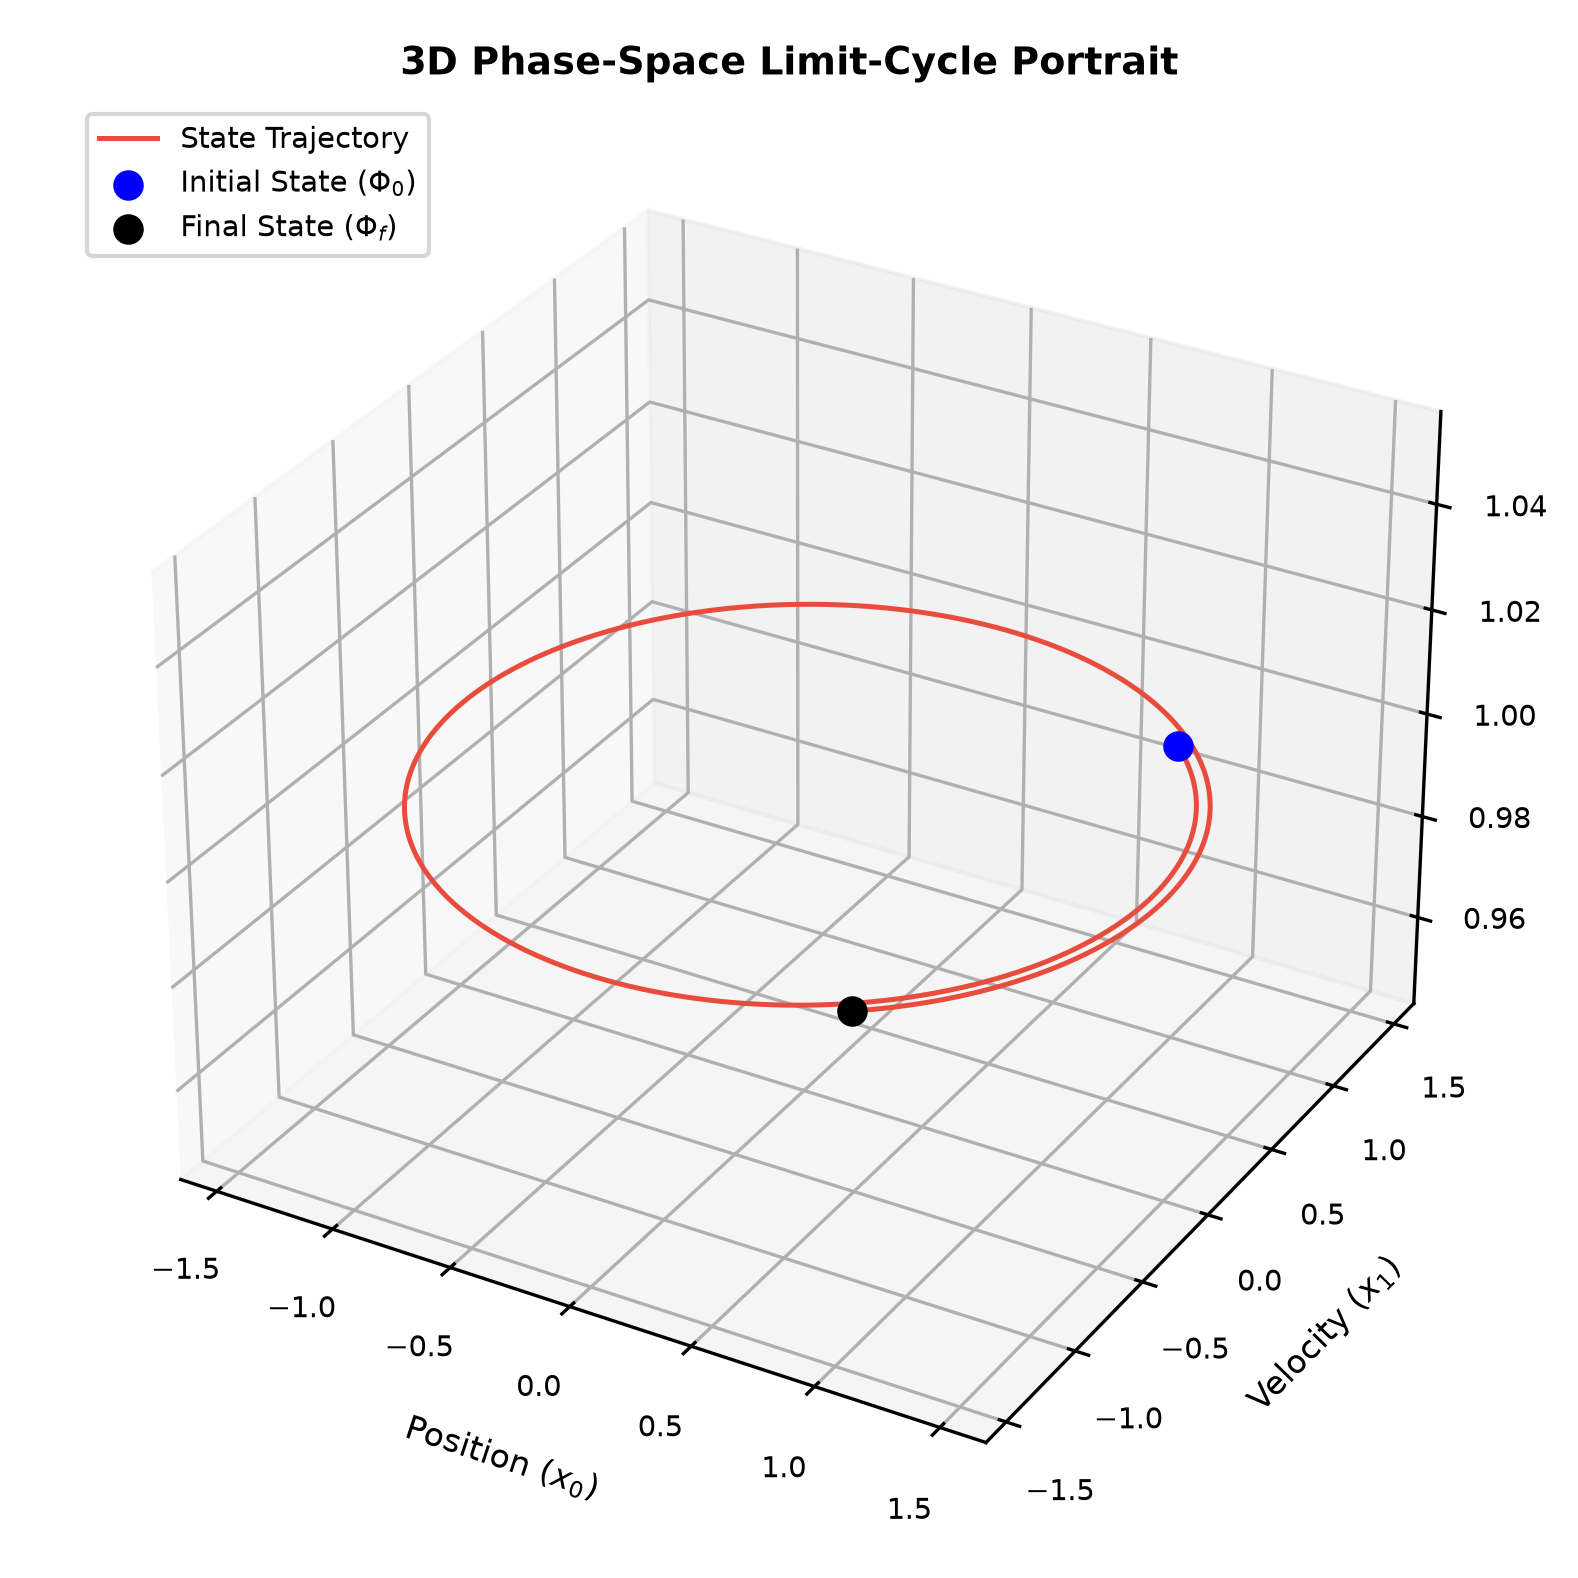
\includegraphics[width=0.5\textwidth]{contents/non-linear-oscillators/the-van-der-pol-oscillator/phase_space_trajectory}
	\caption{Phase Space Trajectory of the Van der Pol Oscillator showing convergence toward the stable limit cycle.}
	\label{fig:vanderpol_phase}
\end{figure}

\section{2D Evolution Plot}
\begin{figure}[ht]
	\centering
	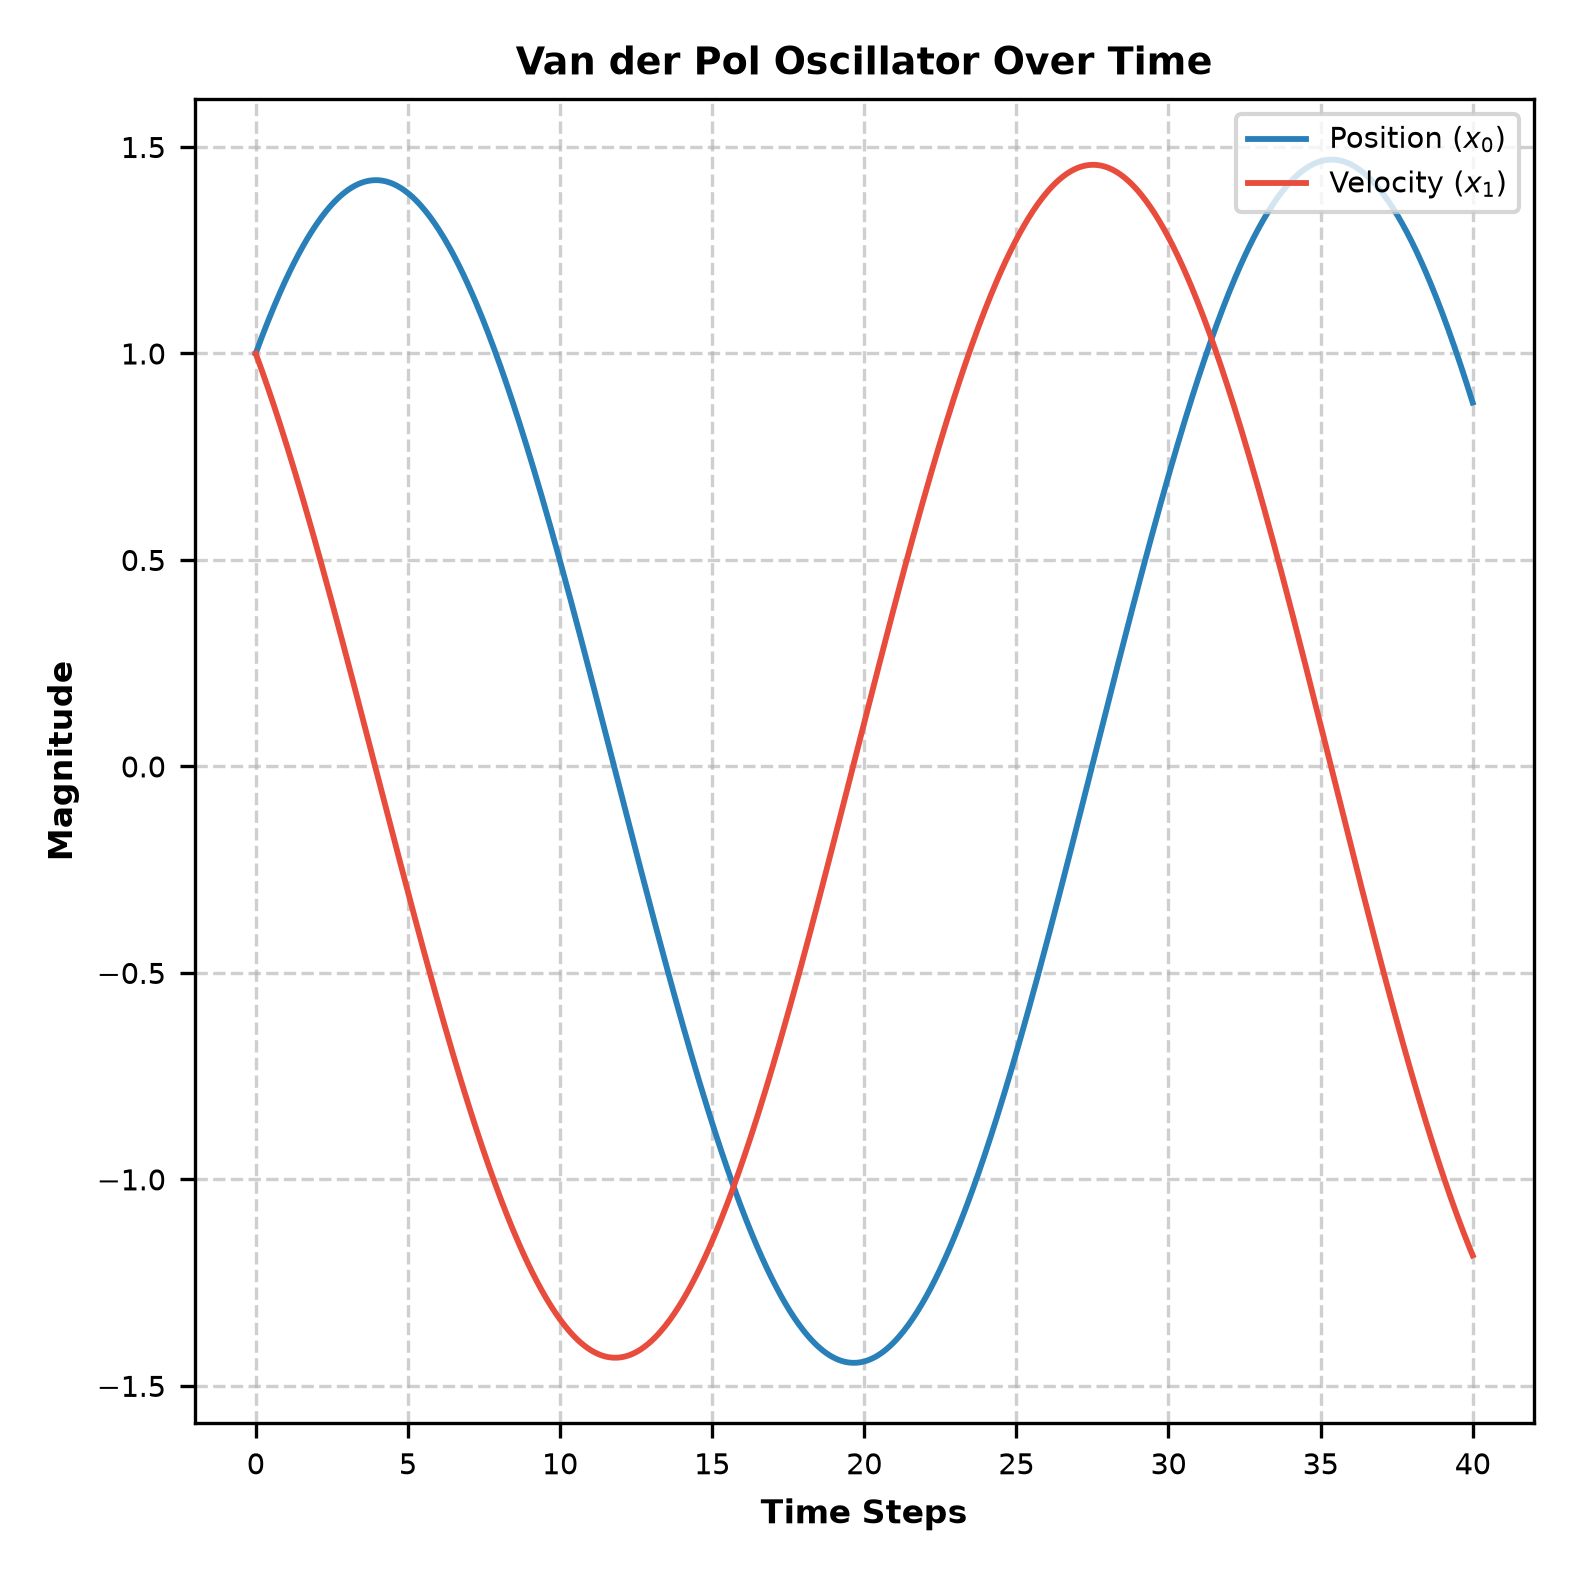
\includegraphics[width=0.5\textwidth]{contents/non-linear-oscillators/the-van-der-pol-oscillator/system_evolution}
	\caption{2D System Evolution displaying temporal relaxation oscillation waveforms.}
	\label{fig:vanderpol_evolution}
\end{figure}

\clearpage
\section{Analysis of the Output}
The SDCM solver correctly captures the energy balancing act of the nonlinear damping term. Starting from an arbitrary initial displacement, the trajectory spirals onto a unique closed limit cycle, maintaining steady periodic oscillations without amplitude drift.

\section{Conclusion}
The Van der Pol oscillator demonstrates the efficacy of the SDCM framework in isolating and maintaining stable limit cycles in non-conservative systems.